\documentclass[final]{beamer}

\usepackage{polyglossia}
\setmainlanguage{english}
\setotherlanguages{russian,czech} % \textlang{russian}{ы}

% 84.1 x 118.9 cm % 120 cm high and 85 cm wide
%\usepackage[size=custom,width=84.1,height=118.9,scale=1.4]{beamerposter}
\usepackage[orientation=portrait,size=a0,scale=1.2]{beamerposter}

\usetheme{gemini}
\usecolortheme{gemini}
\usepackage{graphicx}
\usepackage{booktabs}
\usepackage{tikz}
\usepackage{pgfplots}
\pgfplotsset{compat=1.14}

% If you have N columns, choose \sepwidth and \colwidth such that
% (N+1)*\sepwidth + N*\colwidth = \paperwidth
%\newlength{\sepwidth}
%\newlength{\colwidth}
%\setlength{\sepwidth}{0.025\paperwidth}
%\setlength{\colwidth}{0.3\paperwidth}

\newlength{\sepwidth}
\newlength{\colwidth}
\setlength{\sepwidth}{0.025\paperwidth}
\setlength{\colwidth}{0.47\paperwidth}

\newcommand{\separatorcolumn}{\begin{column}{\sepwidth}\end{column}}

\title{\textit{Pinus sylvestris} L. drought stress reaction thresholds are captured by both intra- and inter-annual variation in xylem morphology}

\author{Sergei Mikhailov \inst{1-3} \and Marek Fajstavr \inst{1,2} \and Petr Horáček \inst{1,2}}

\institute[MendelU]{\inst{1} Department of Xylogenesis and Biomass Allocation, CzechGlobe, CZ \samelineand \inst{2} Department of Wood Science and Technology, Mendel University in Brno, CZ \samelineand \inst{3} Laboratory of Ecology of Plant Communities, Komarov Botanical Institute of the Russian Academy of Sciences, Saint Petersburg, RU}
%\institute[MendelU]{\inst{1} Department of Xylogenesis and Biomass Allocation, CzechGlobe, Brno, Czech Republic \samelineand \inst{2} Department of Wood Science and Technology, Mendel University in Brno, Brno, Czech Republic \samelineand \inst{3} Laboratory of Ecology of Plant Communities, Komarov Botanical Institute of the Russian Academy of Sciences, Saint Petersburg, Russian Federation}

\footercontent{
  
\includegraphics[height=5cm]{pics/qr}
  {\LaTeX} \& R code in git repo \hfill
  \hspace{0cm} XIM5 2022, Würzburg \hfill
  %\href{https://www.github.com/aplantc0}{github.com/aplantc0}
  
\includegraphics[height=5cm]{pics/logo_mendelu}
  
\includegraphics[height=5cm]{pics/logo_czechglobe}
  %\href{mailto:mikhailov.s@czechglobe.cz}{mikhailov.s@czechglobe.cz}
  % (can be left out to remove footer)
}

% use this to include logos on the left and/or right side of the header:
%\logoleft{
\includegraphics[height=7cm]{pics/logo_mendelu}}
%\logoright{
\includegraphics[height=5cm]{pics/logo_czechglobe}}

\begin{document}

\begin{frame}[t]
\begin{columns}[t]

%\separatorcolumn

\begin{column}{\colwidth}

    \begin{alertblock}{Hypetheses and questions}
        %\large
        We studied Scots pine xylem formation on 2 research plots (150--350 m asl), representing managed Scots pine stands aged 40 (\textbf{Young}) and 100 (\textbf{Old}) years in the south of the Czech Republic during the two successive years of 2020 \& 2021.
        \begin{itemize}
            \item What are the variation ranges of Scots pine cell morphology parameters under the drought stress? To quantify
            \item To what extent Scots pine trees can withstand water deficit stress, and is cellular level of observation better allows to identify it?
            \item What the numerical thresholds in number, radial dimensions of tracheids and tree-ring width, up to which these variables can decline without the tree dieback?
            \item Is the same mechanism of drought stress reaction in Scots pine revealed regardless of the tree age?
        \end{itemize}
    \end{alertblock}

    \begin{block}{Methodology}
        \heading{Dendroclimatology}
            Retrospective whole-tree livespan time-series analysis (12 trees). Tree ring width (TRW) measurements, cross-dating, standardization by fitting the Hugershoff function, chronology building (Figure 3); climate--growth relationships: responce and correlation function with T\textsubscript{avg}, P\textsubscript{sum}, SPEI\textsubscript{1}.
        \heading{Xylogenesis}
            Following the xylem formation dynamics (6 trees). Weekly microcore sampling, sample preparation, number of cells in each phase was measured under the light microscope with x10--x20 magnification, cell formation phases: i) enlarging; ii) cell-wall thickening; iii) maturation.
        \heading{Xylem morphology}
            Quantitative wood anatomy (6 trees). Capture image of the two last fully formed annual rings (2020 \& 2021), image batch processing with ImageMagick, measurements with ImageJ: continuous sequence of lumen diameter and cell wall thickness (Figure 1.
        \heading{Climatic data}
            Daily (site): T, RH, \Psi\textsubscript{Soil}, sap flow. Monthly (external): T\textsubscript{avg}, P\textsubscript{sum}, SPEI\textsubscript{1}.
            \begin{figure}
                \centering 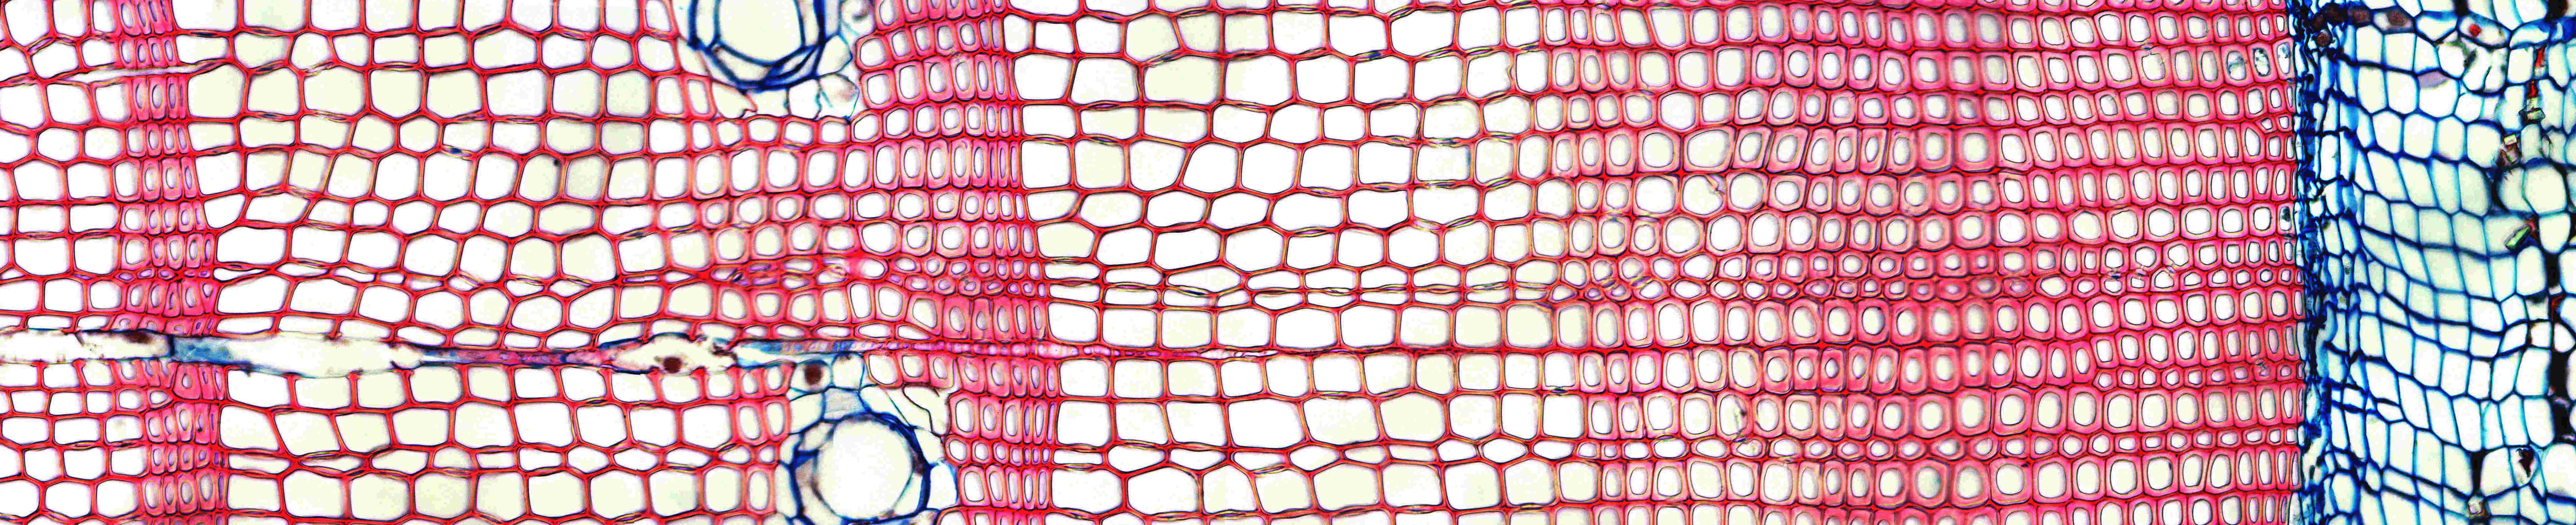
\includegraphics[width=1\textwidth]{pics/sob}
                \caption{Two consequtive annual rings of 2020 \& 2021 (Old stand), x20 magnification. Cambium is on the right \rightarrow}
            \end{figure}
    \end{block}

    \begin{block}{Drought stress}
            \begin{figure}
                \centering \includegraphics[width=1\textwidth]{pics/sap}
                \caption{Sap flow during two years of 2020 \& 2021}
            \end{figure}
    \end{block}

\end{column}

%\separatorcolumn

\begin{column}{\colwidth}

    \begin{block}{Results}
        \heading{Tree ring width}
            \begin{figure}
                \centering \includegraphics[width=1\textwidth]{pics/hf}
                \caption{Raw (left) and indexed (right) TRW chronologies. HF -- the Huggershoff function curve fitting the age trend; RWI -- ring width index}
            \end{figure}
        \heading{Xylo- \& morphogenesis}
            \begin{figure}
                \centering 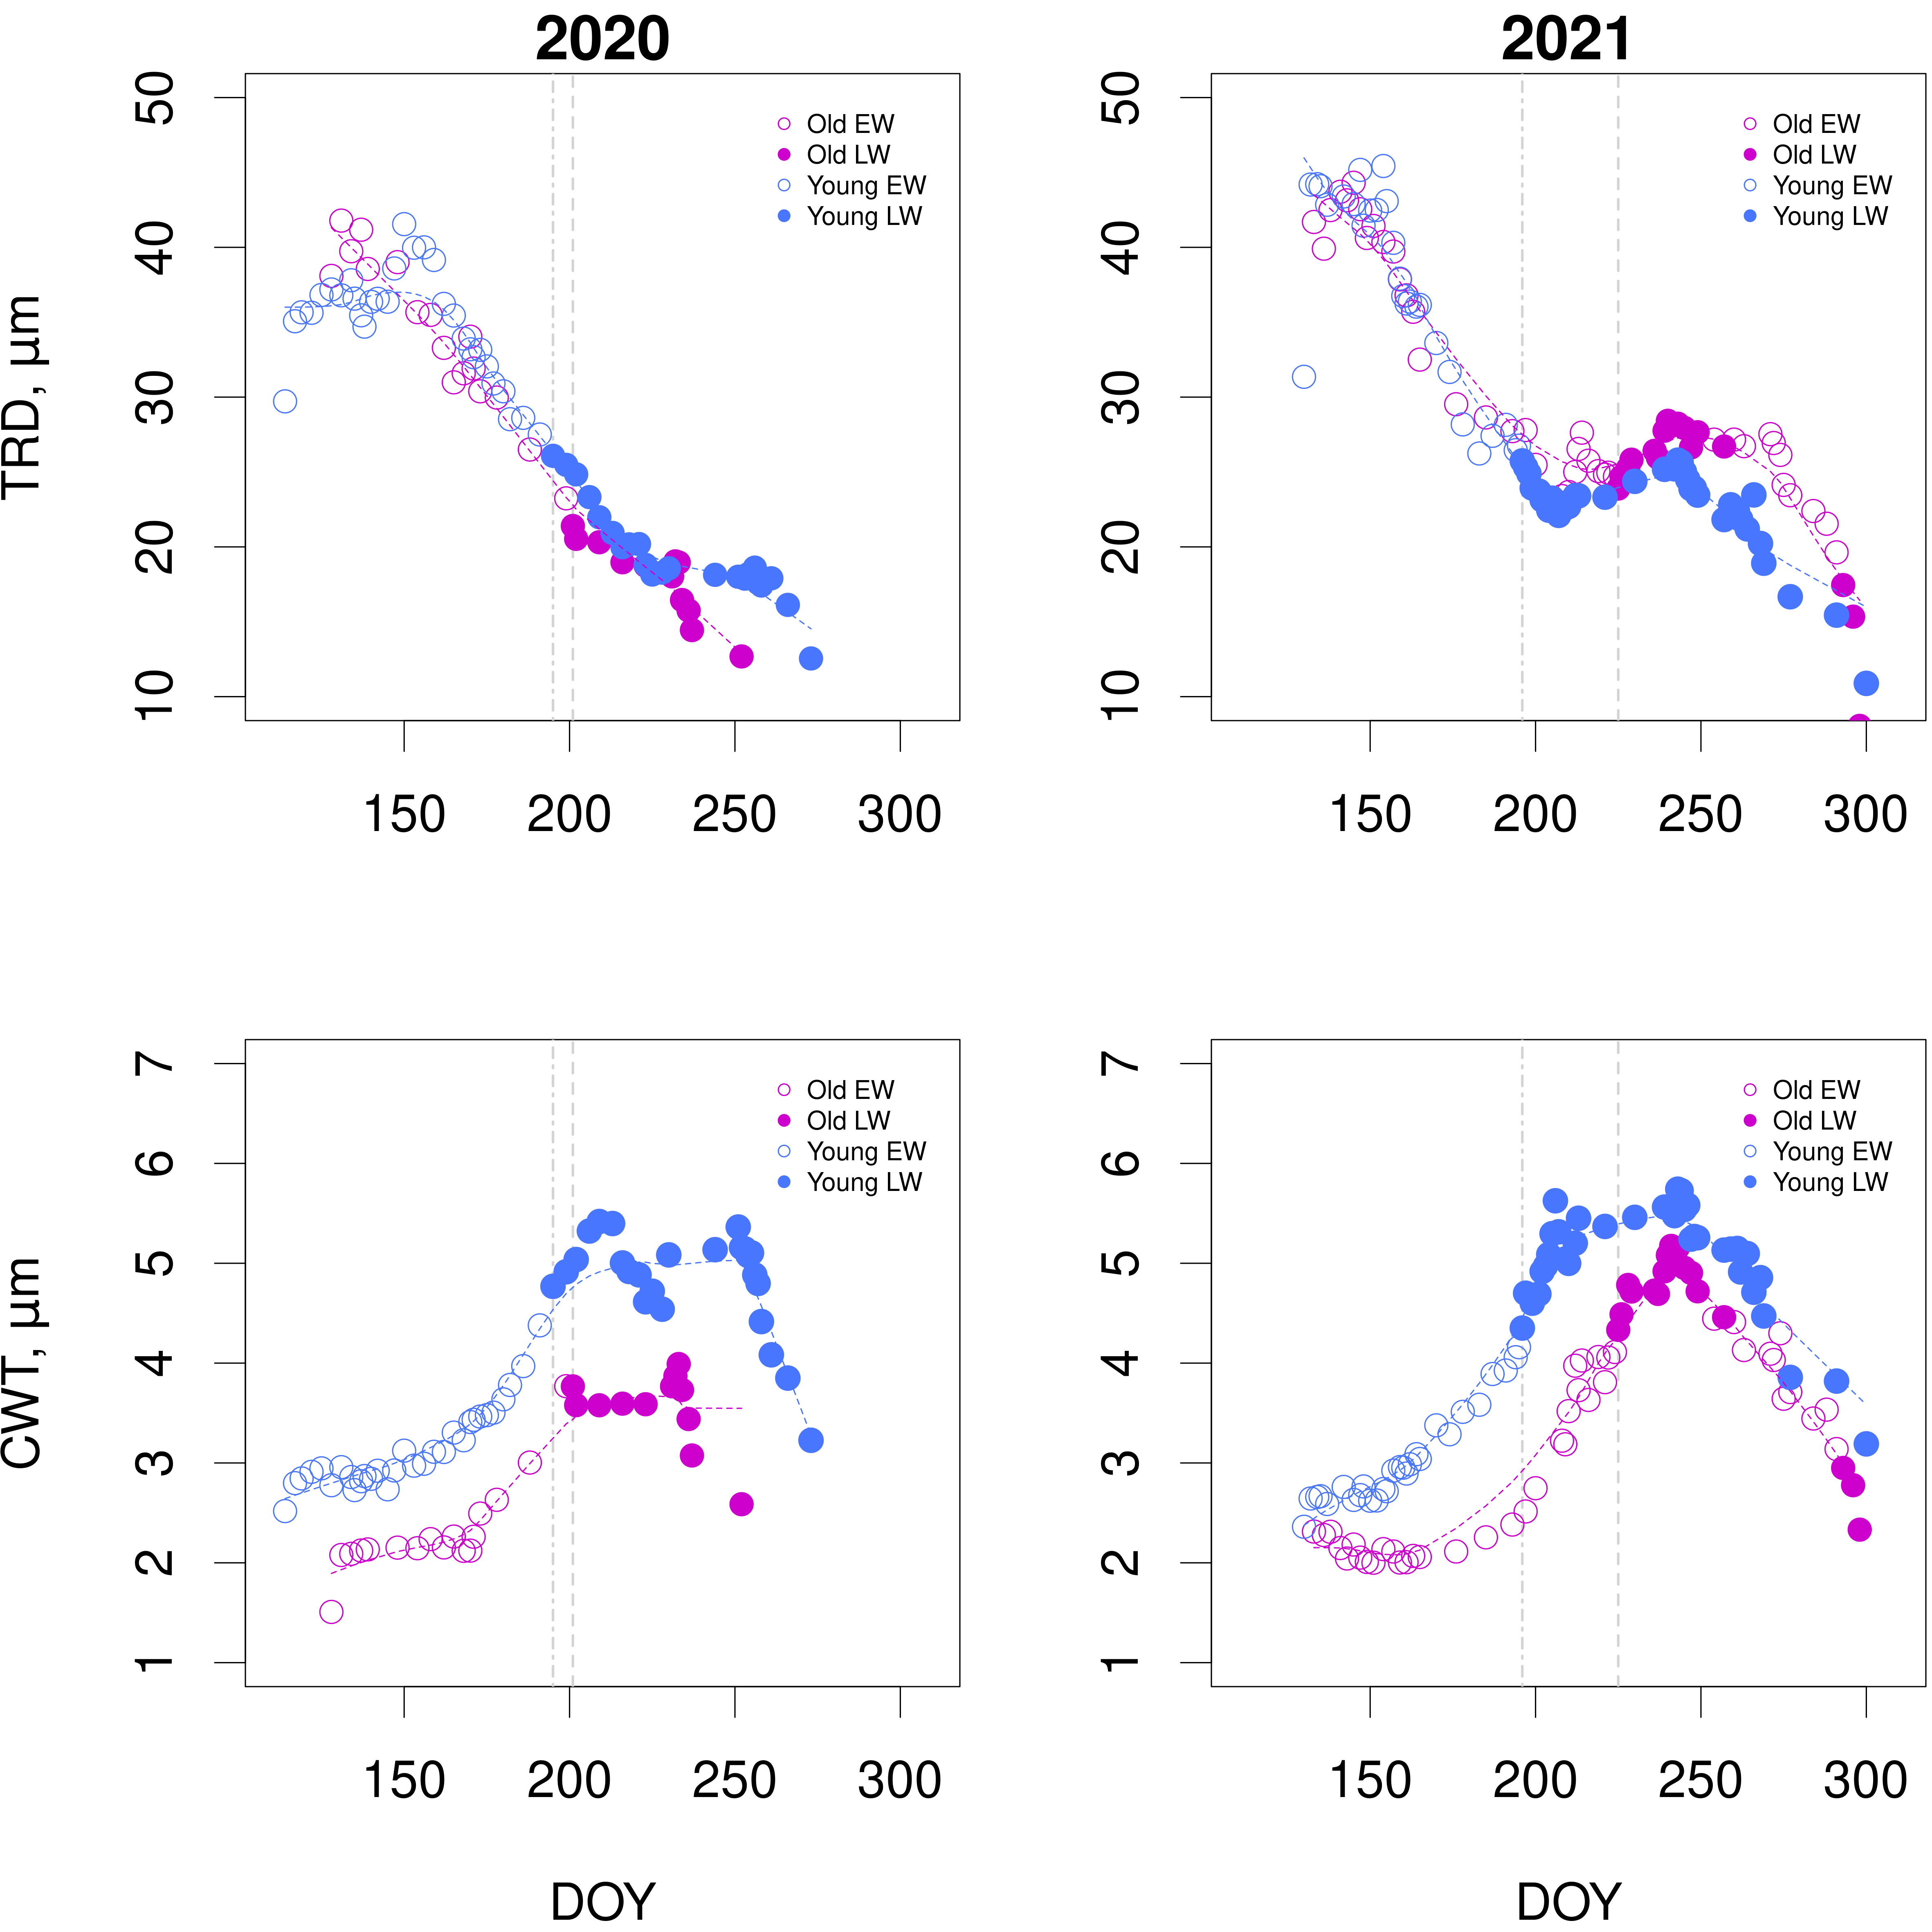
\includegraphics[width=1\textwidth]{pics/xmg}
                \caption{TRD -- tracheid radial diameter, CWT -- cell wall thickness, DOY -- day of the year when the process of cell wall thickening began (i.e., TRD has already been defined), EW -- early wood, LW -- late wood (classified based on Mork's criteria}
            \end{figure}
    \end{block}

    \begin{block}{Conclusions}
        \begin{itemize}
            \item TRD, CWT varies between
            \item Number of cells
            \item Number of cells
            \item Number of cells
        \end{itemize}
    \end{block}

\end{column}
\end{columns}

\begin{columns}[c]
    \begin{column}{.95\paperwidth}
    \begin{block}{What is next?}
        \raggedleft
        \begin{itemize}
            \item To study wood formation dynamics in the following years on more Scots pine plots with different age structure in the Czech Republic, and then\dots
            \item {\dots}To study xylem morphology and climate--growth relationships on the upper limit of species distribution in northern taiga primary (undisturbed) forest communities 
        \end{itemize}
    \end{block}
\end{column}

%\separatorcolumn

\end{columns}
\end{frame}

\end{document}
